\textbf{Activity}: Commits in Git, submitted, merged and abandoned reviews in Gerrit and opened and closed issues in Launchpad.


\begin{tabular}{p{7cm} p{5cm}}
    \vspace{0pt} 
    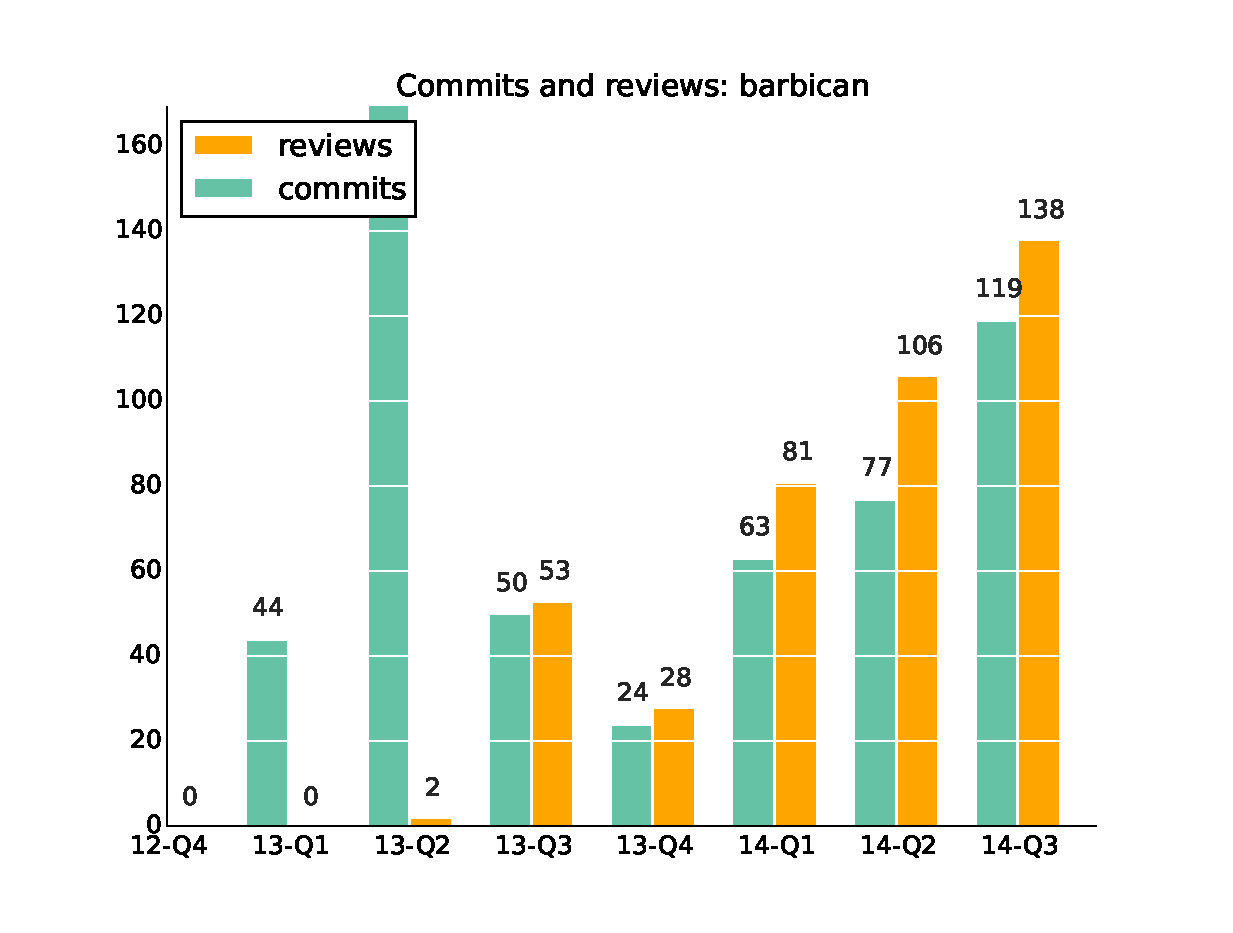
\includegraphics[scale=.35]{figs/commitsbarbican.eps}
    & 
    \vspace{0pt}
    \begin{tabular}{l|r|r|}%
    \bfseries Period & \bfseries Commits & \bfseries Reviews % specify table head
    \csvreader[head to column names]{data/commitsbarbican.csv}{}% use head of csv as column names
    {\\\labels & \commits & \submitted}
    \end{tabular}
\end{tabular}

\begin{tabular}{p{7cm} p{5cm}}
    \vspace{0pt} 
    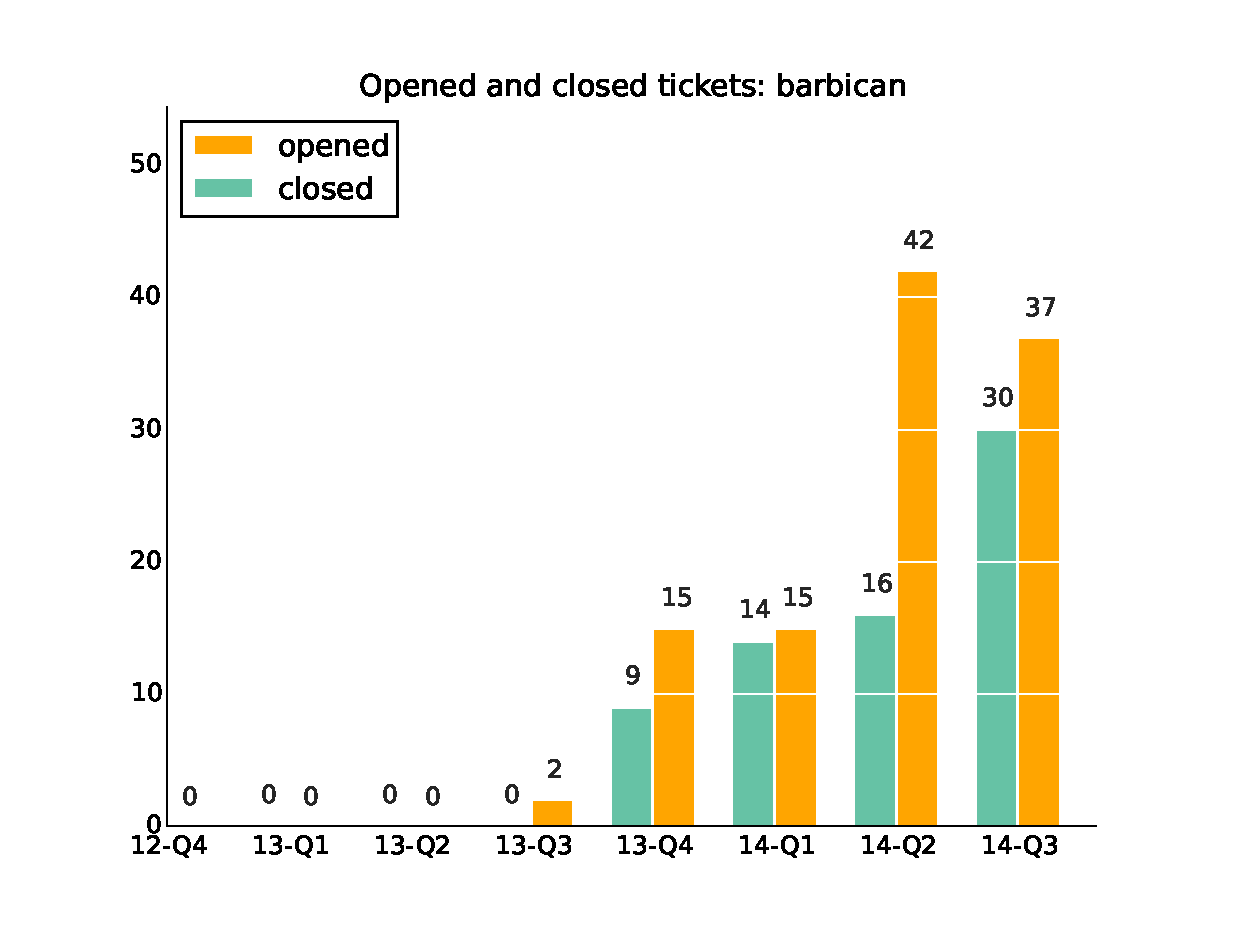
\includegraphics[scale=.35]{figs/closedbarbican.eps}
    & 
    \vspace{0pt}
    \begin{tabular}{l|r|r|}%
    \bfseries Period & \bfseries Closed & \bfseries Opened
    \csvreader[head to column names]{data/closedbarbican.csv}{}% use head of csv as column names
    {\\\labels & \closed & \opened}
    \end{tabular}
\end{tabular}

\begin{tabular}{p{7cm} p{5cm}}
    \vspace{0pt} 
    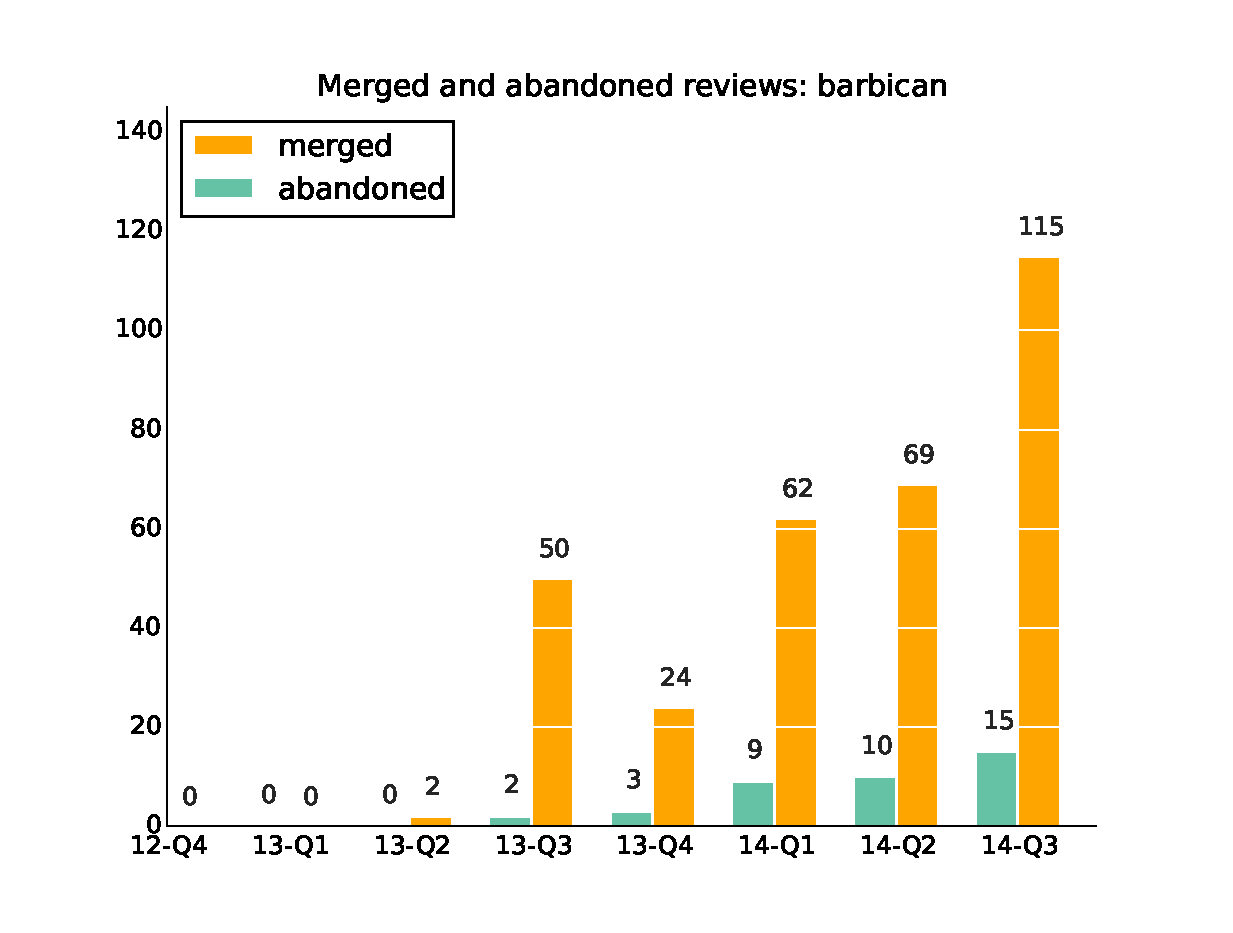
\includegraphics[scale=.35]{figs/submitted_reviewsbarbican.eps}
    & 
    \vspace{0pt}
    \begin{tabular}{l|r|r|}%
    \bfseries Period & \bfseries Merged & \bfseries Abandoned % specify table head
    \csvreader[head to column names]{data/submitted_reviewsbarbican.csv}{}% use head of csv as column names
    {\\\labels & \merged & \abandoned}
    \end{tabular}
\end{tabular}


\section{Community}
Active core reviewers in Gerrit, active authors in Git, top authors and organizations in the last quarter



\begin{tabular}{p{7cm} p{5cm}}
    \vspace{0pt} 
    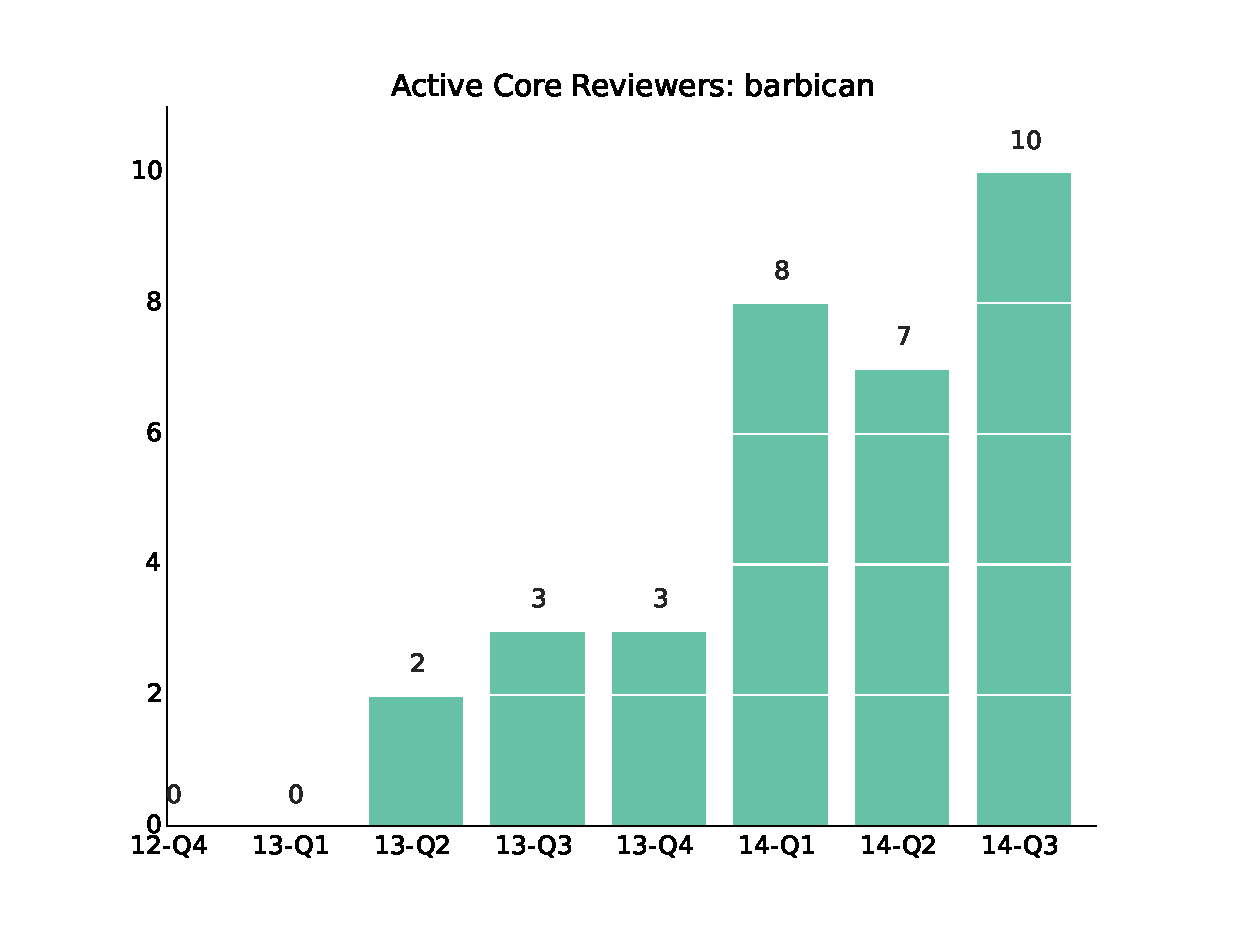
\includegraphics[scale=.35]{figs/active_core_scrbarbican.eps}
    & 
    \vspace{0pt}
    \begin{tabular}{l|l}%
    \bfseries Period & \bfseries Active Core % specify table head
    \csvreader[head to column names]{data/active_core_scrbarbican.csv}{}% use head of csv as column names
    {\\\labels & \activecorereviewers}
    \end{tabular}
\end{tabular}

\begin{tabular}{p{7cm} p{5cm}}
    \vspace{0pt} 
    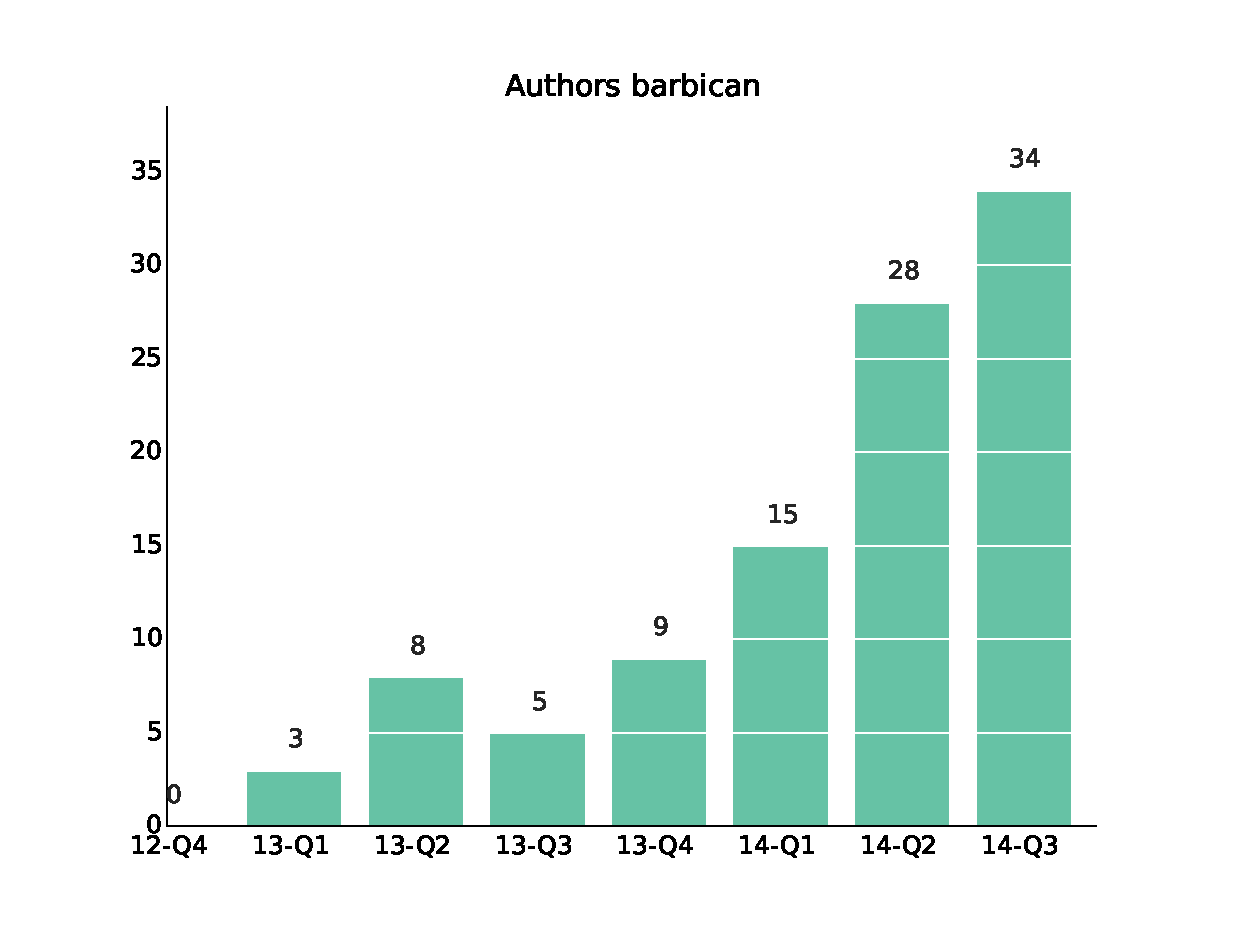
\includegraphics[scale=.35]{figs/authorsbarbican.eps}
    & 
    \vspace{0pt}
    \begin{tabular}{l|l}%
    \bfseries Period & \bfseries Authors % specify table head
    \csvreader[head to column names]{data/authorsbarbican.csv}{}% use head of csv as column names
    {\\\labels & \authors}
    \end{tabular}
\end{tabular}

\begin{tabular}{p{7cm} p{5cm}}
    \vspace{0pt}
\begin{tabular}{l|l}%
    \bfseries Commit (s) & \bfseries Author % specify table head
    \csvreader[head to column names]{data/scm_top_authors_project_barbican.csv}{}% use head of csv as column names
    {\\\hline\csvcoli&\csvcolii}% specify your coloumns here
\end{tabular}
&
\vspace{0pt}
\begin{tabular}{l|l}%
    \bfseries Commit (s) & \bfseries Organizations % specify table head
    \csvreader[head to column names]{data/scm_top_companies_project_barbican.csv}{}% use head of csv as column names
    {\\\hline\csvcoli&\csvcolii}% specify your coloumns here
\end{tabular}
\end {tabular}

\textbf{Process}: Efficiency closing changesets and tickets, time to review (mean and median), number of patchests (iterations)
per changeset and study on the time waiting for a reviewer or submitter action in the patchset review process.


\begin{tabular}{p{7cm} p{5cm}}
    \vspace{0pt} 
    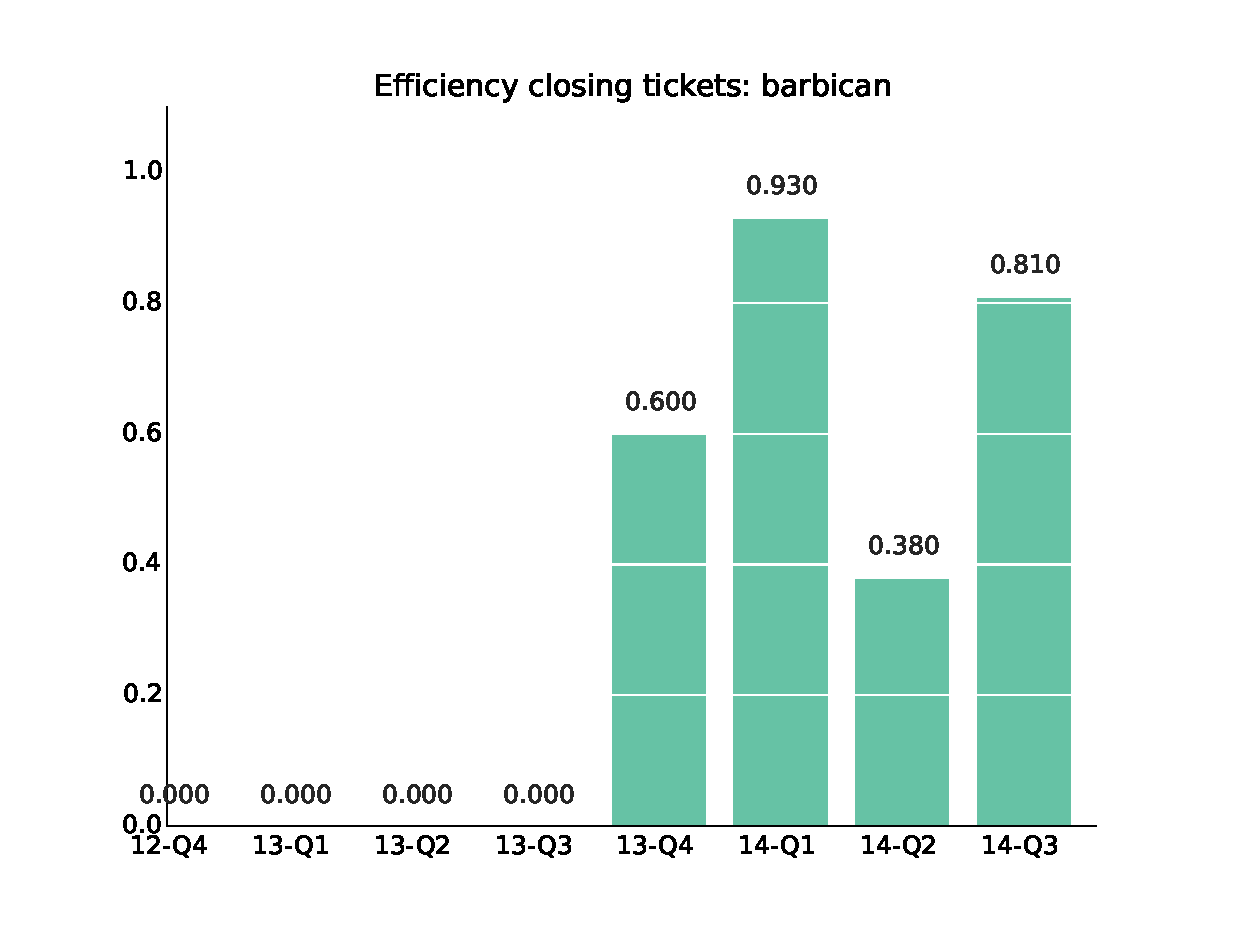
\includegraphics[scale=.35]{figs/bmibarbican.eps}
    & 
    \vspace{0pt}
    \begin{tabular}{l|l}%
    \bfseries Period & \bfseries Closed/Opened % specify table head
    \csvreader[head to column names]{data/bmibarbican.csv}{}% use head of csv as column names
    {\\\labels & \bmi}
    \end{tabular}
\end{tabular}

\begin{tabular}{p{7cm} p{5cm}}
    \vspace{0pt} 
    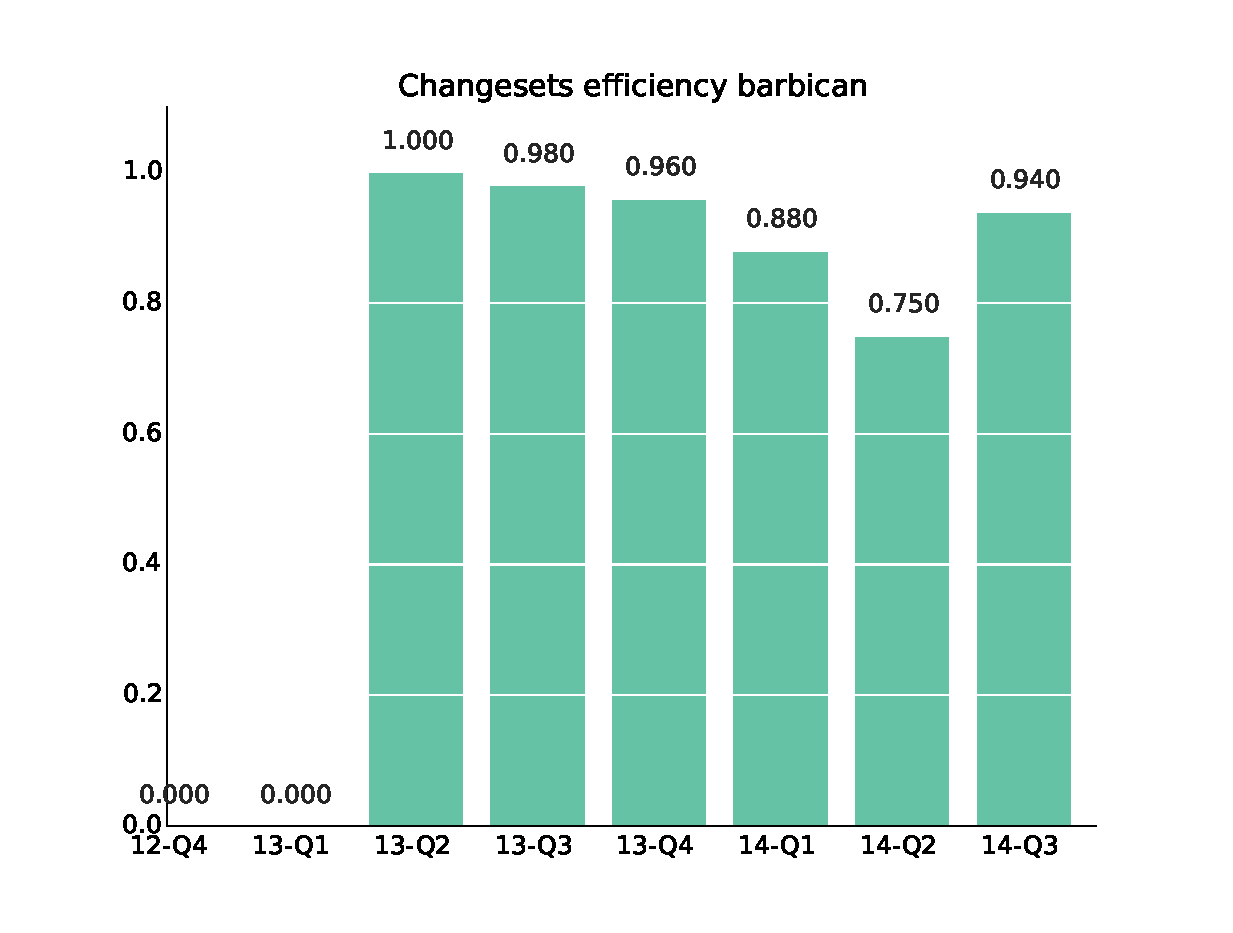
\includegraphics[scale=.35]{figs/bmiscrbarbican.eps}
    & 
    \vspace{0pt}
    \begin{tabular}{l|l}%
    \bfseries Period & \bfseries Closed/Opened % specify table head
    \csvreader[head to column names]{data/submitted_reviewsbarbican.csv}{}% use head of csv as column names
    {\\\labels & \bmi}
    \end{tabular}
\end{tabular}


\begin{tabular}{p{7cm} p{5cm}}
    \vspace{0pt} 
    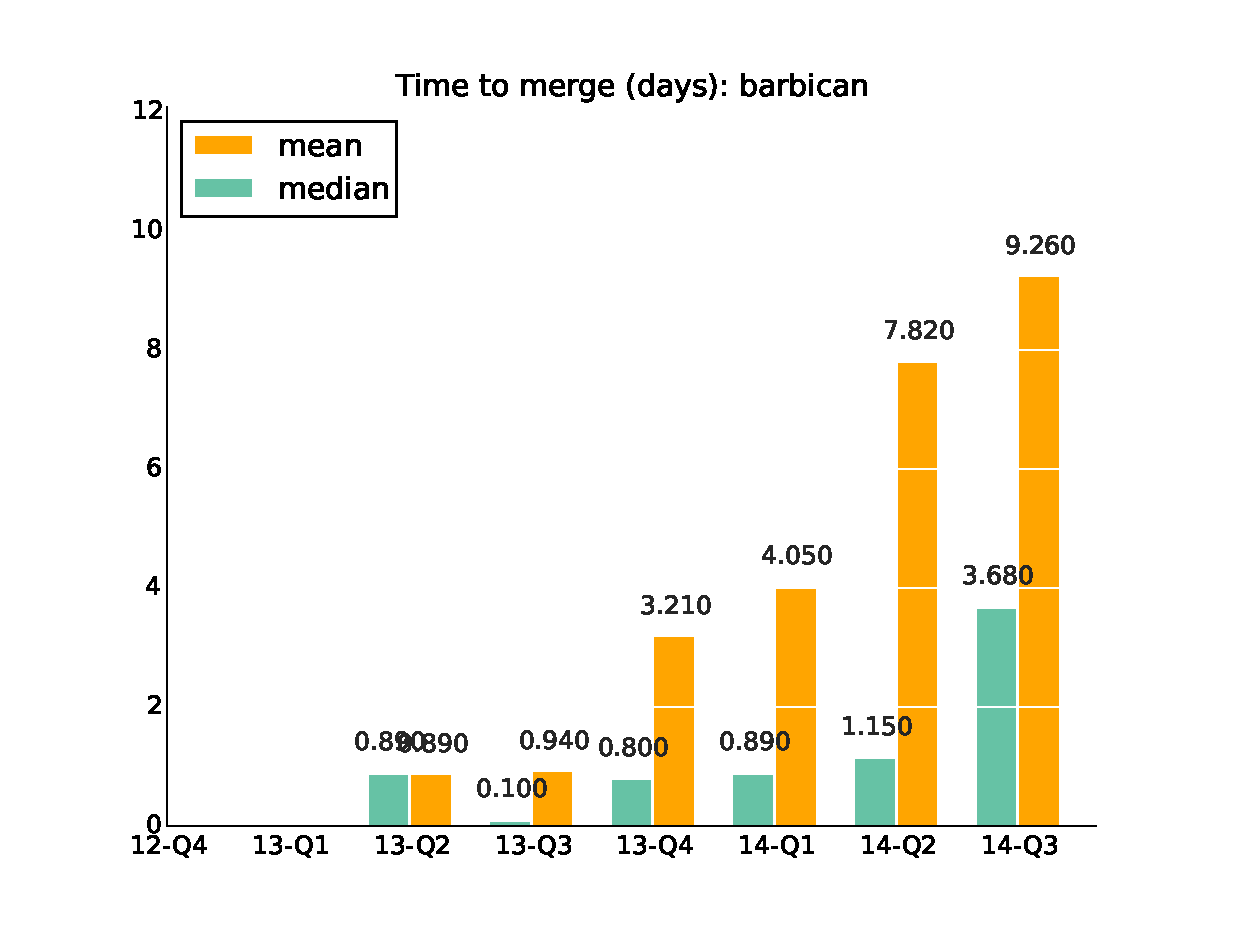
\includegraphics[scale=.35]{figs/timetoreview_medianbarbican.eps}
    & 
    \vspace{0pt}
    \begin{tabular}{l|r|r|}%
    \bfseries Period & \bfseries Median & \bfseries Mean % specify table head
    \csvreader[head to column names]{data/timetoreview_medianbarbican.csv}{}% use head of csv as column names
    {\\\labels & \mediantime & \meantime}
    \end{tabular}
\end{tabular}


\begin{tabular}{p{7cm} p{5cm}}
    \vspace{0pt} 
    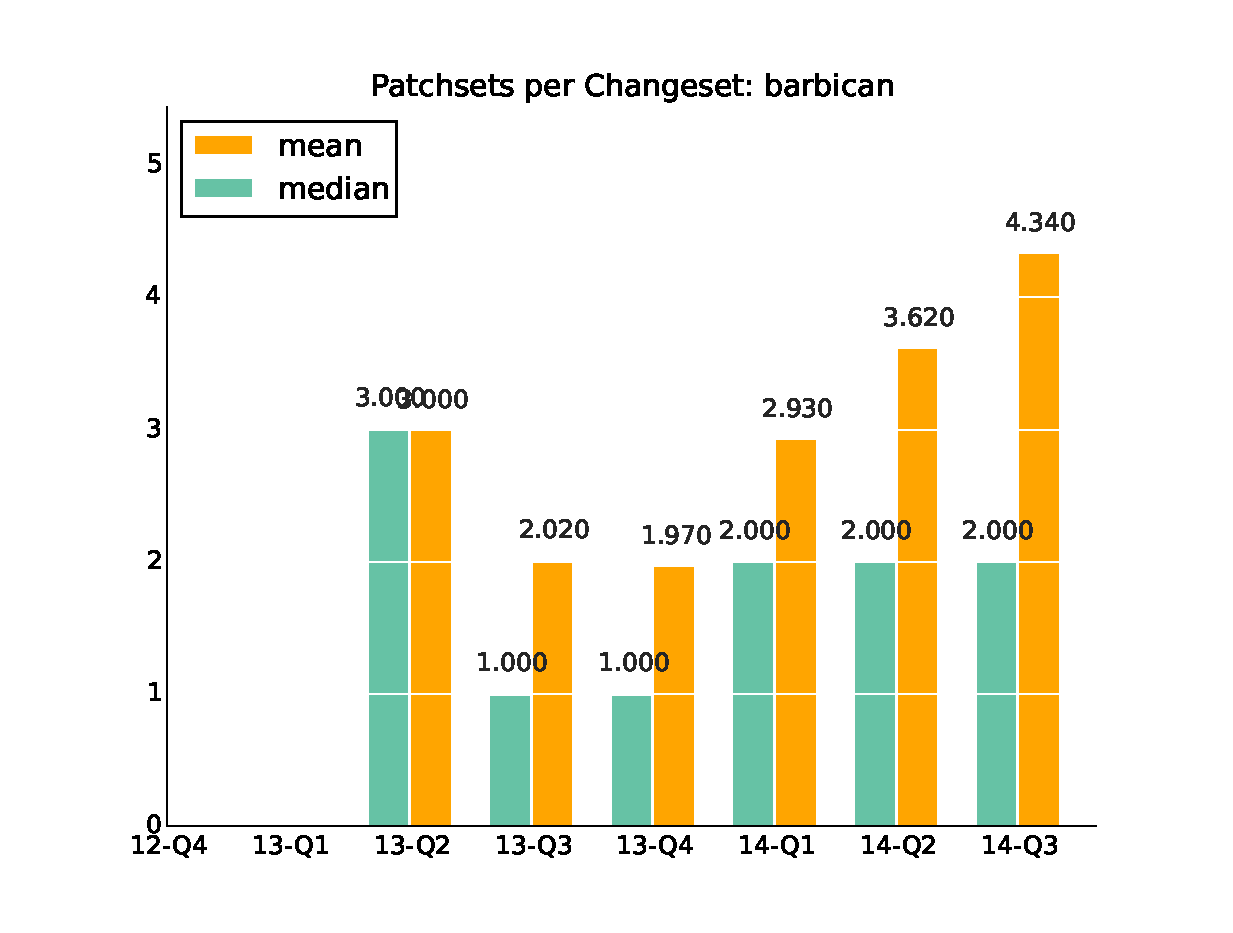
\includegraphics[scale=.35]{figs/patchsets_avgbarbican.eps}
    & 
    \vspace{0pt}
    \begin{tabular}{l|r|r|}%
    \bfseries Period & \bfseries Median & \bfseries Mean % specify table head
    \csvreader[head to column names]{data/scr_patchsets_iterationsbarbican.csv}{}% use head of csv as column names
    {\\\labels & \medianpatchsets & \meanpatchsets}
    \end{tabular}
\end{tabular}

\begin{tabular}{p{7cm} p{5cm}}
    \vspace{0pt} 
    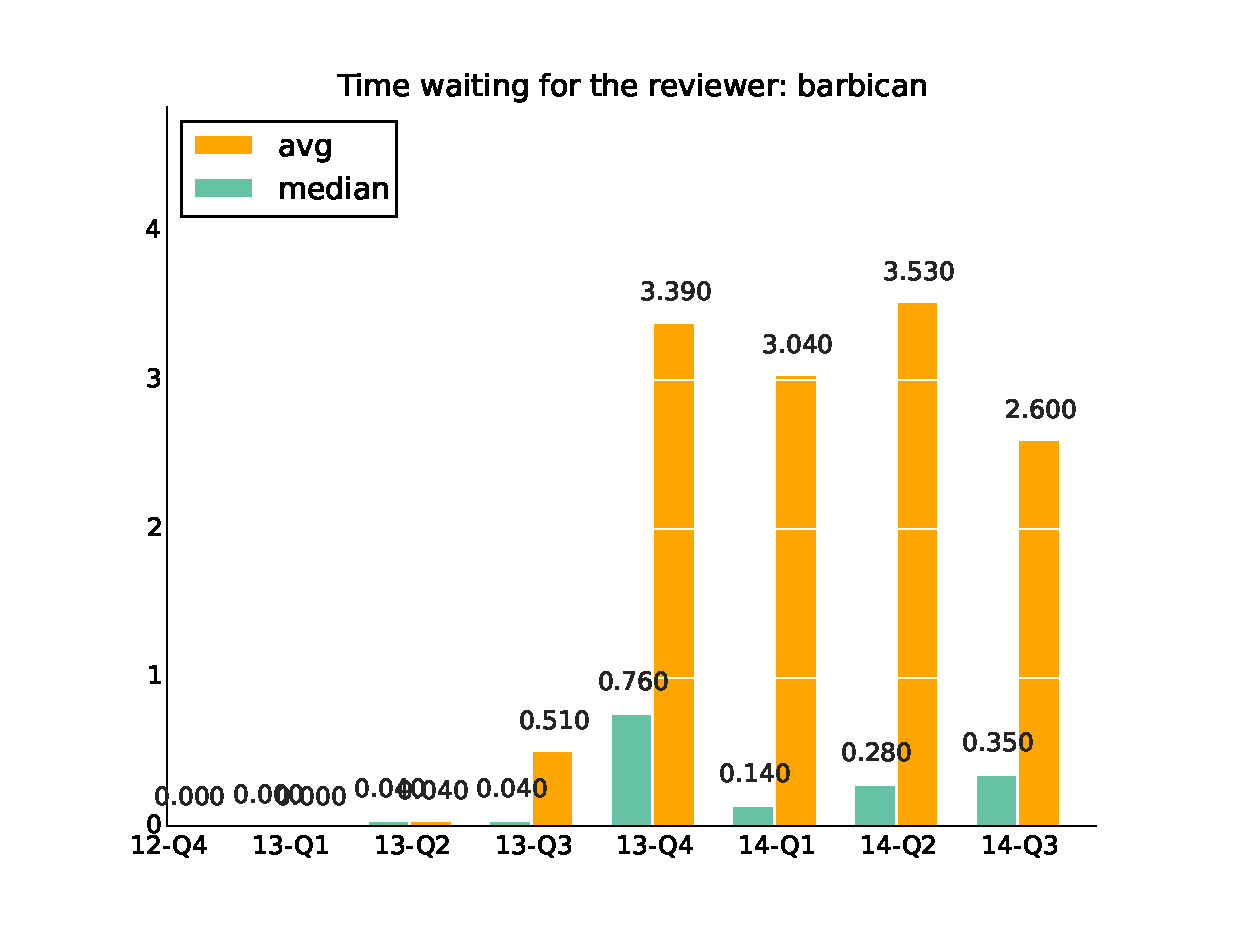
\includegraphics[scale=.35]{figs/waiting4reviewer_avgbarbican.eps}
    & 
    \vspace{0pt}
    \begin{tabular}{l|r|r|}%
    \bfseries Period & \bfseries Median & \bfseries Mean % specify table head
    \csvreader[head to column names]{data/timewaiting4reviewer_medianbarbican.csv}{}% use head of csv as column names
    {\\\labels & \mediantime & \meantime}
    \end{tabular}
\end{tabular}

\begin{tabular}{p{7cm} p{5cm}}
    \vspace{0pt} 
    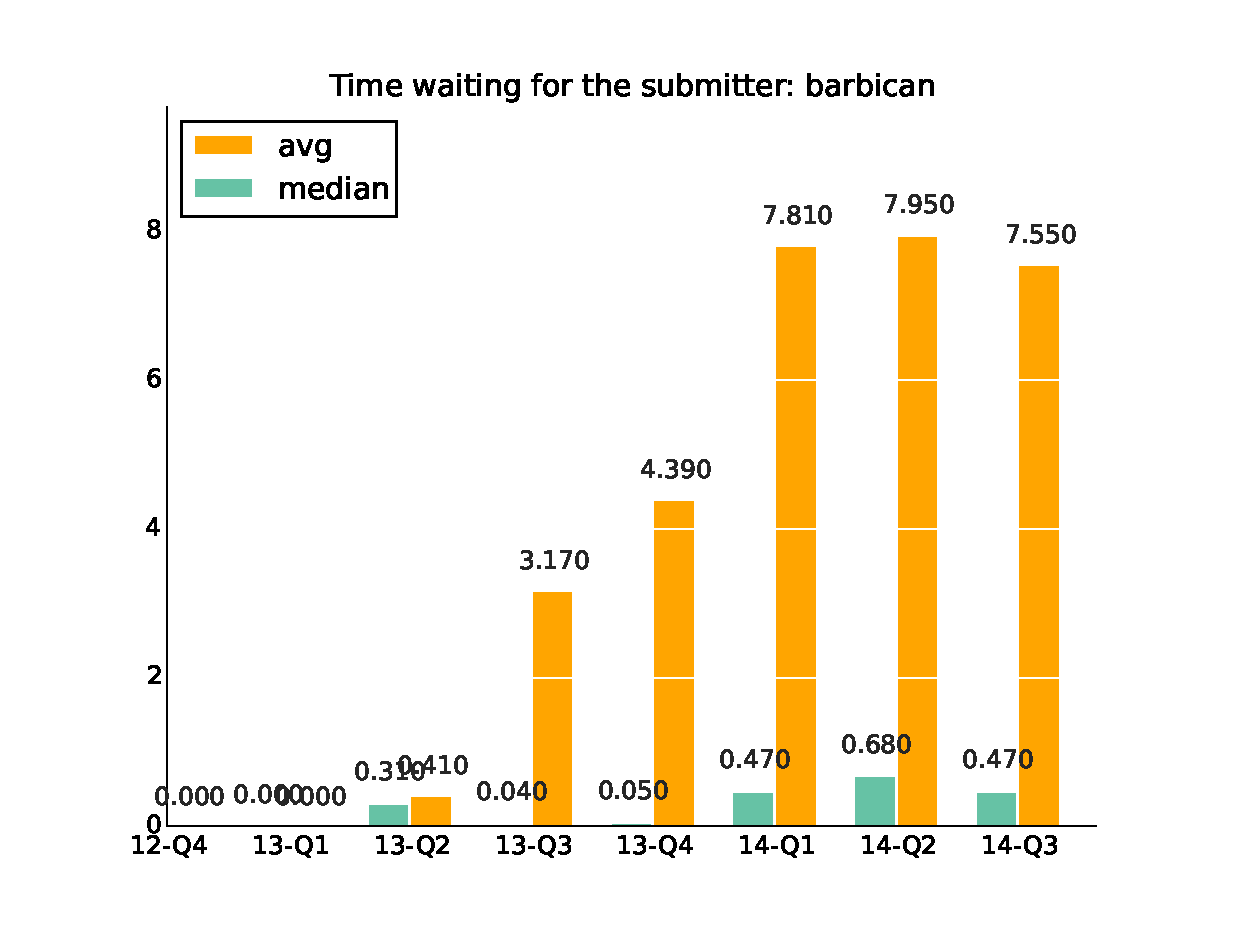
\includegraphics[scale=.35]{figs/waiting4submitter_avgbarbican.eps}
    & 
    \vspace{0pt}
    \begin{tabular}{l|r|r|}%
    \bfseries Period & \bfseries Median & \bfseries Mean % specify table head
    \csvreader[head to column names]{data/timewaiting4submitter_medianbarbican.csv}{}% use head of csv as column names
    {\\\labels & \mediantime & \meantime}
    \end{tabular}
\end{tabular}

